\begin{figure*}[!t]
\centering
\subfloat[][Model size]{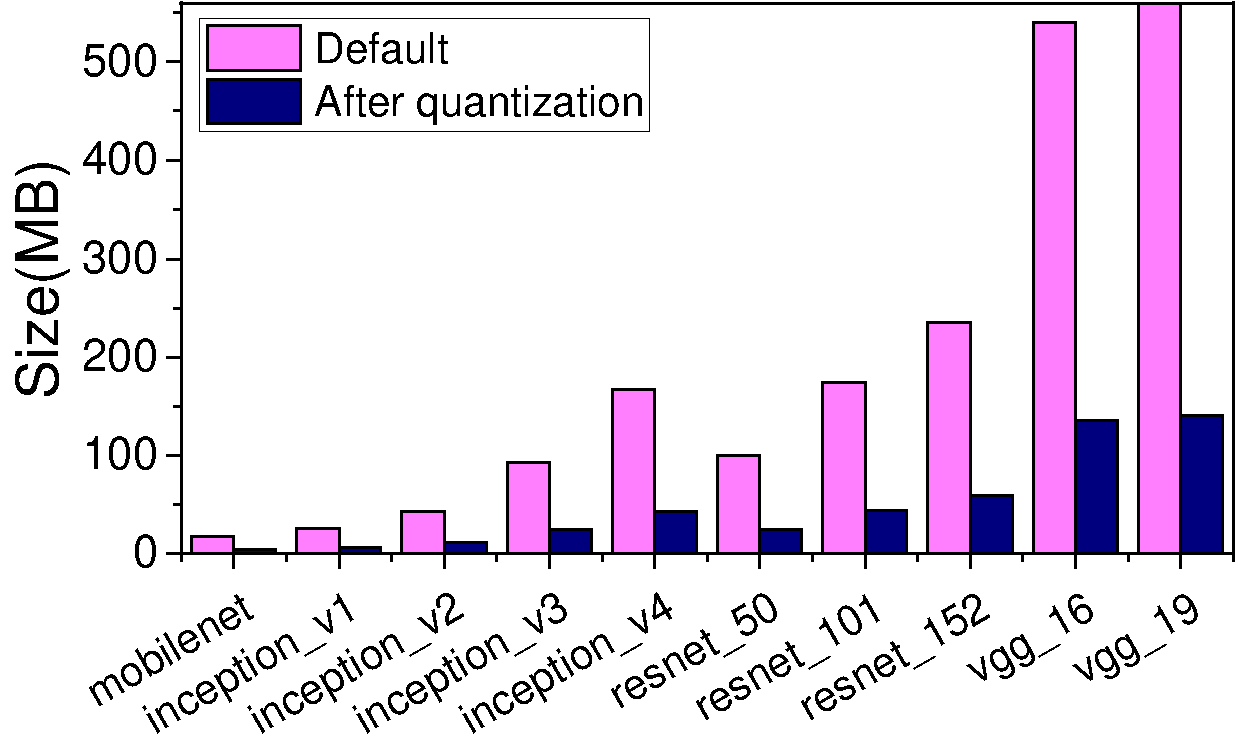
\includegraphics[width=0.3\textwidth]{figure/quan_size.pdf}}
\hfill
\subfloat[][Inference time]{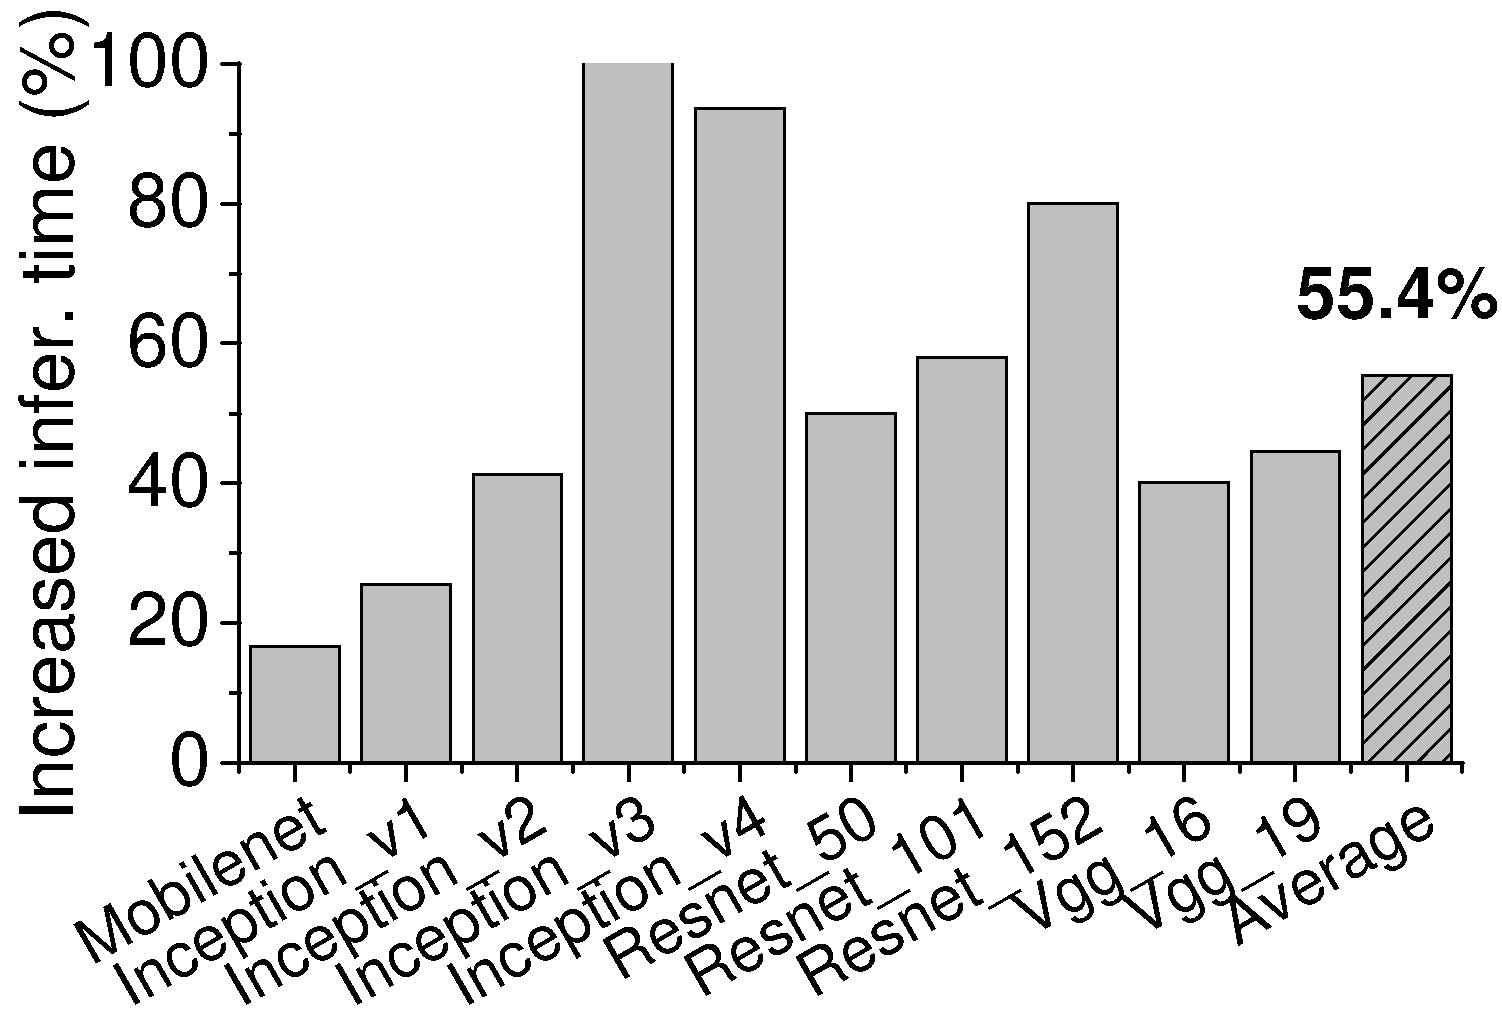
\includegraphics[width=0.3\textwidth]{figure/quan_time.pdf}}
\hfill
\subfloat[][Accuracy]{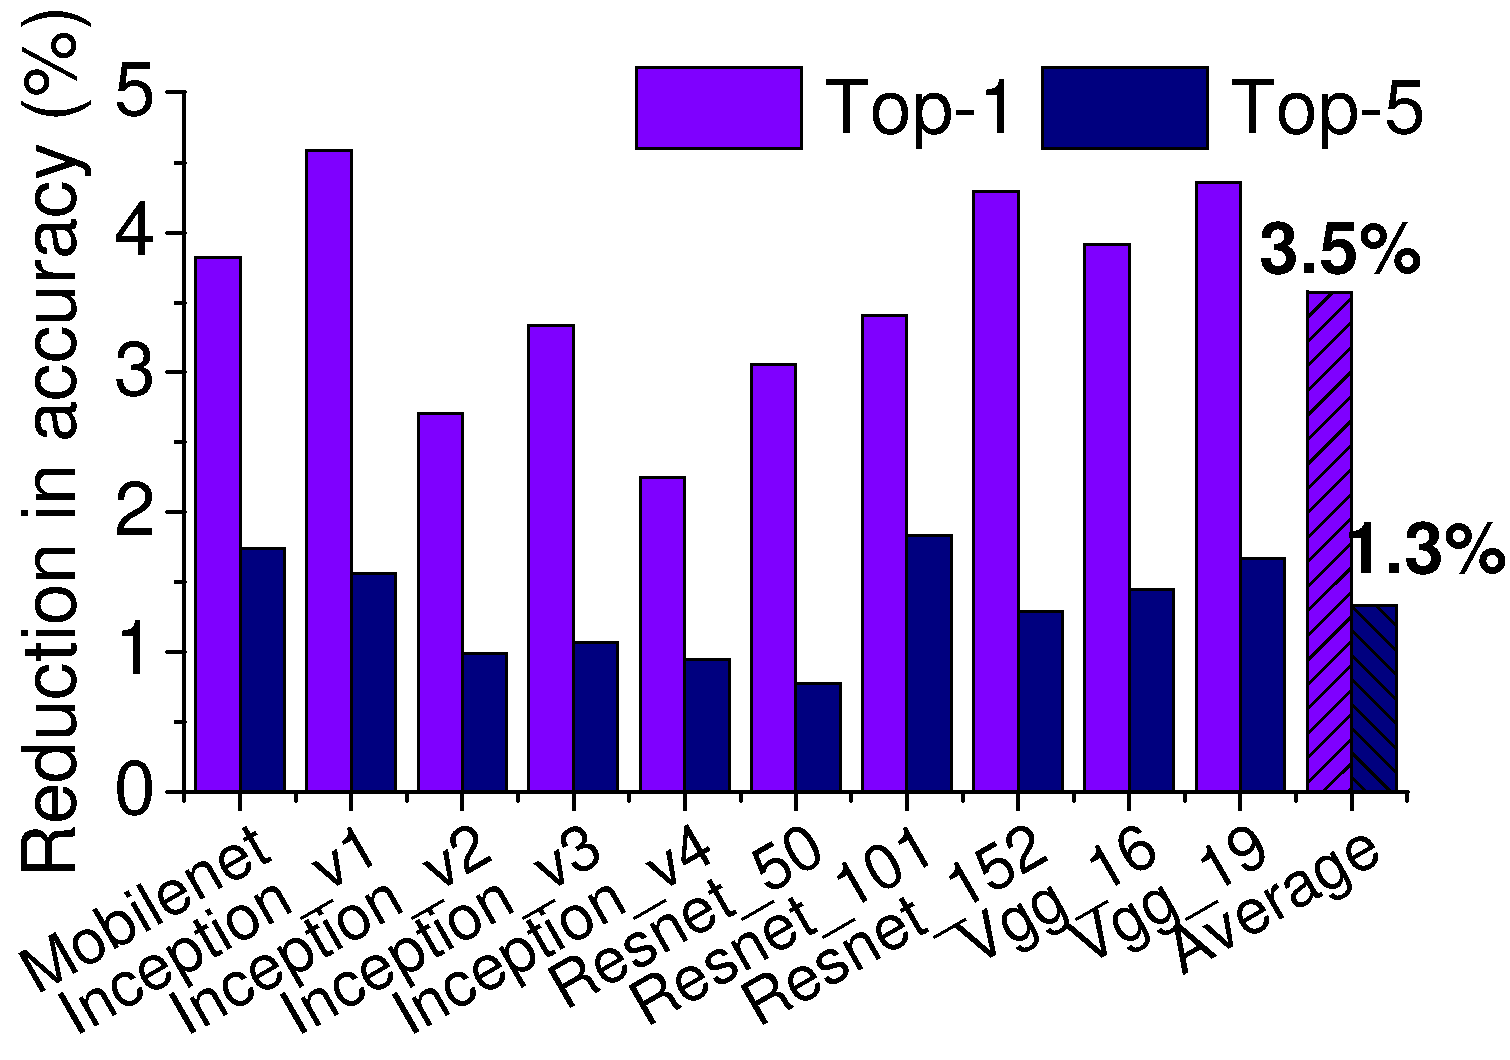
\includegraphics[width=0.3\textwidth]{figure/top1_5_quan.pdf}}
\hfill
\subfloat[][Power consumption]{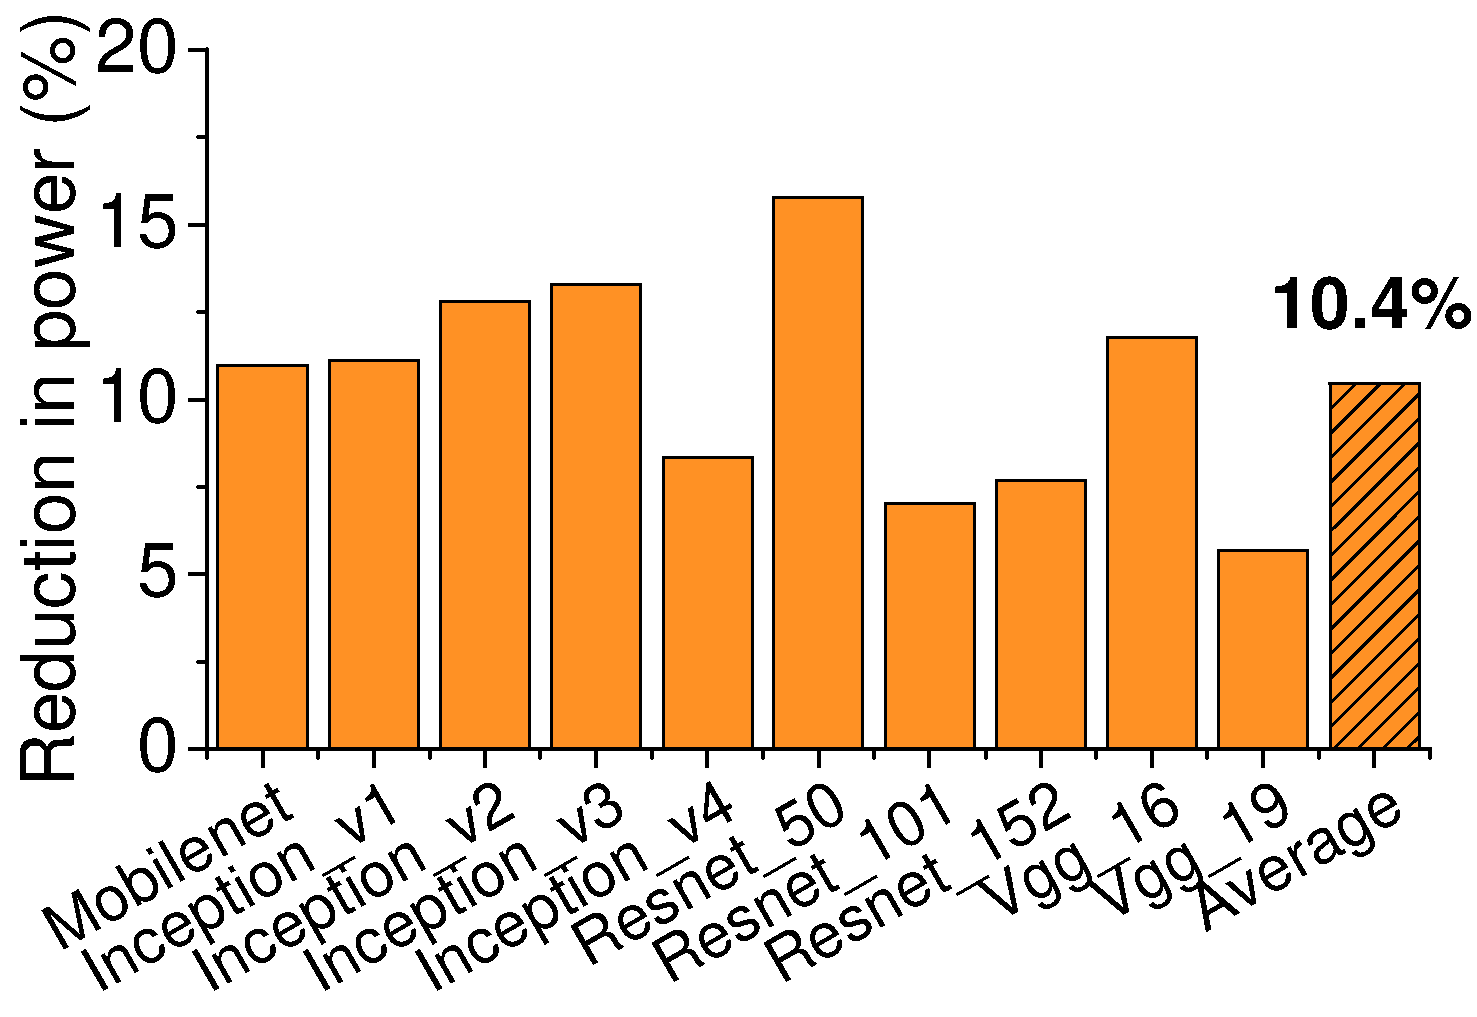
\includegraphics[width=0.3\textwidth]{figure/quan_power.pdf}}
\hfill
\subfloat[][Energy consumption]{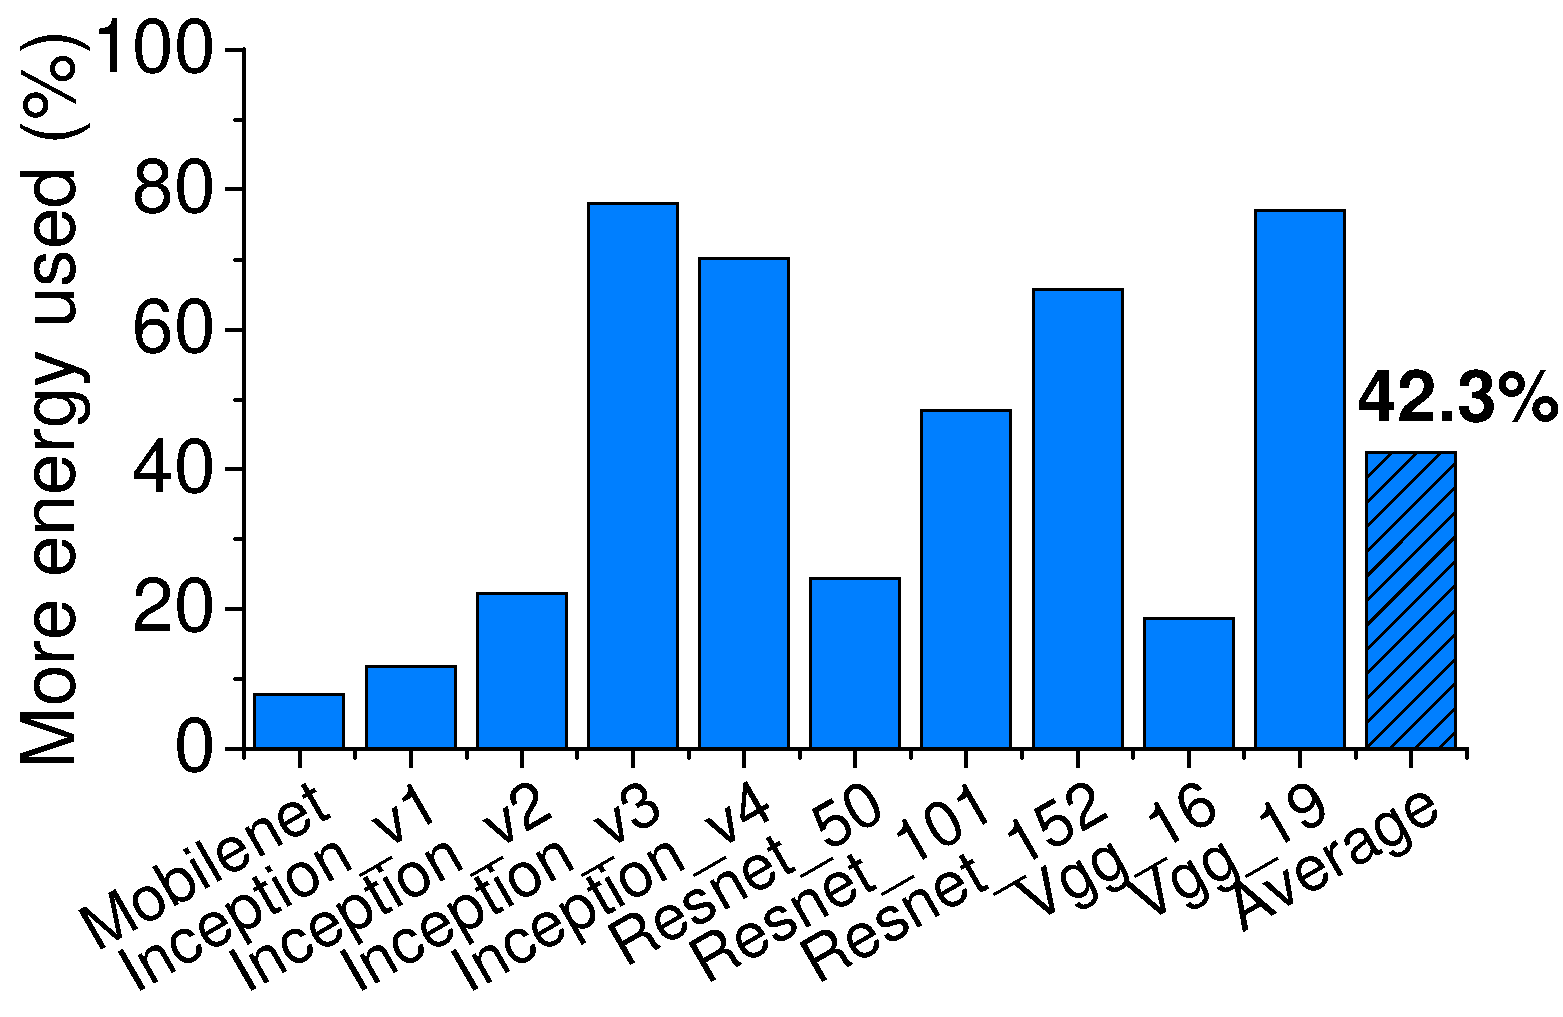
\includegraphics[width=0.3\textwidth]{figure/quan_energy.pdf}}
\hfill

\caption{The achieved model size (a) inference time (b) accuracy (c) power consumption (d)
energy consumption (e) and F1 score (e) before and after the compression by \quantization.
The compression technique to use depends on the optimization target.\FIXME{f1 score later}}
\label{fig:analy_quan}
\end{figure*}


\begin{figure*}[!t]
\centering
\subfloat[][Model size]{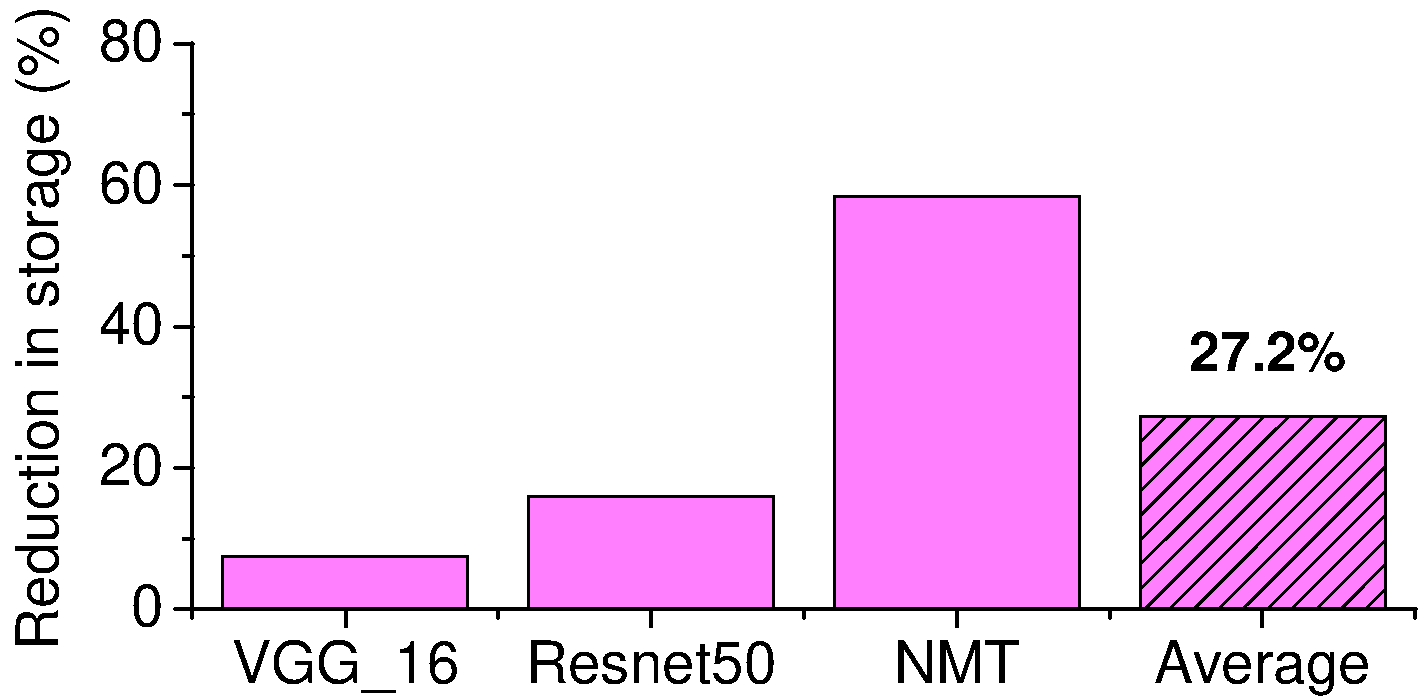
\includegraphics[width=0.3\textwidth]{figure/prun_size.pdf}}
\hfill
\subfloat[][Inference time]{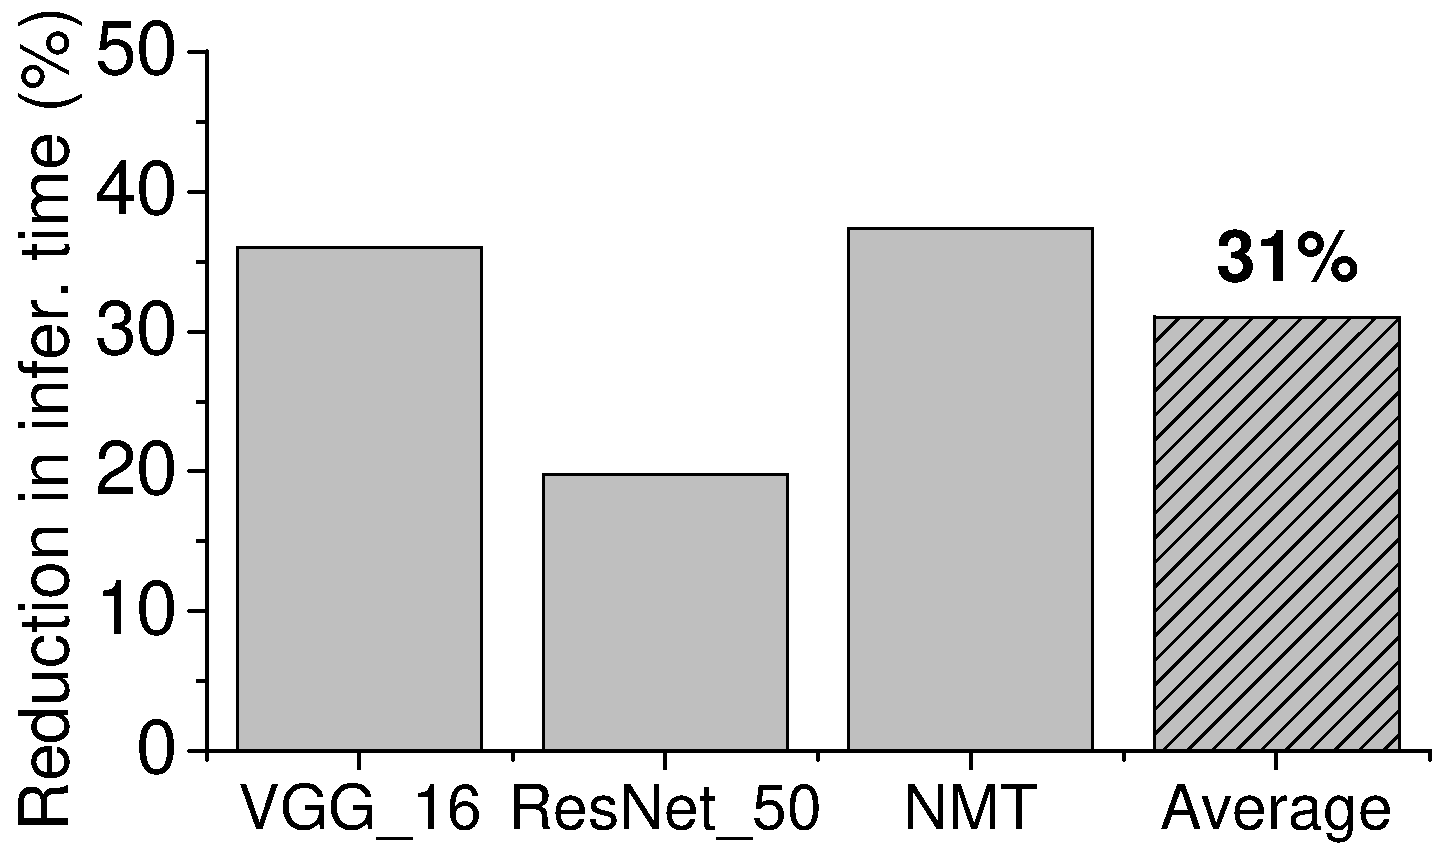
\includegraphics[width=0.3\textwidth]{figure/prun_time.pdf}}
\hfill
\subfloat[][Accuracy]{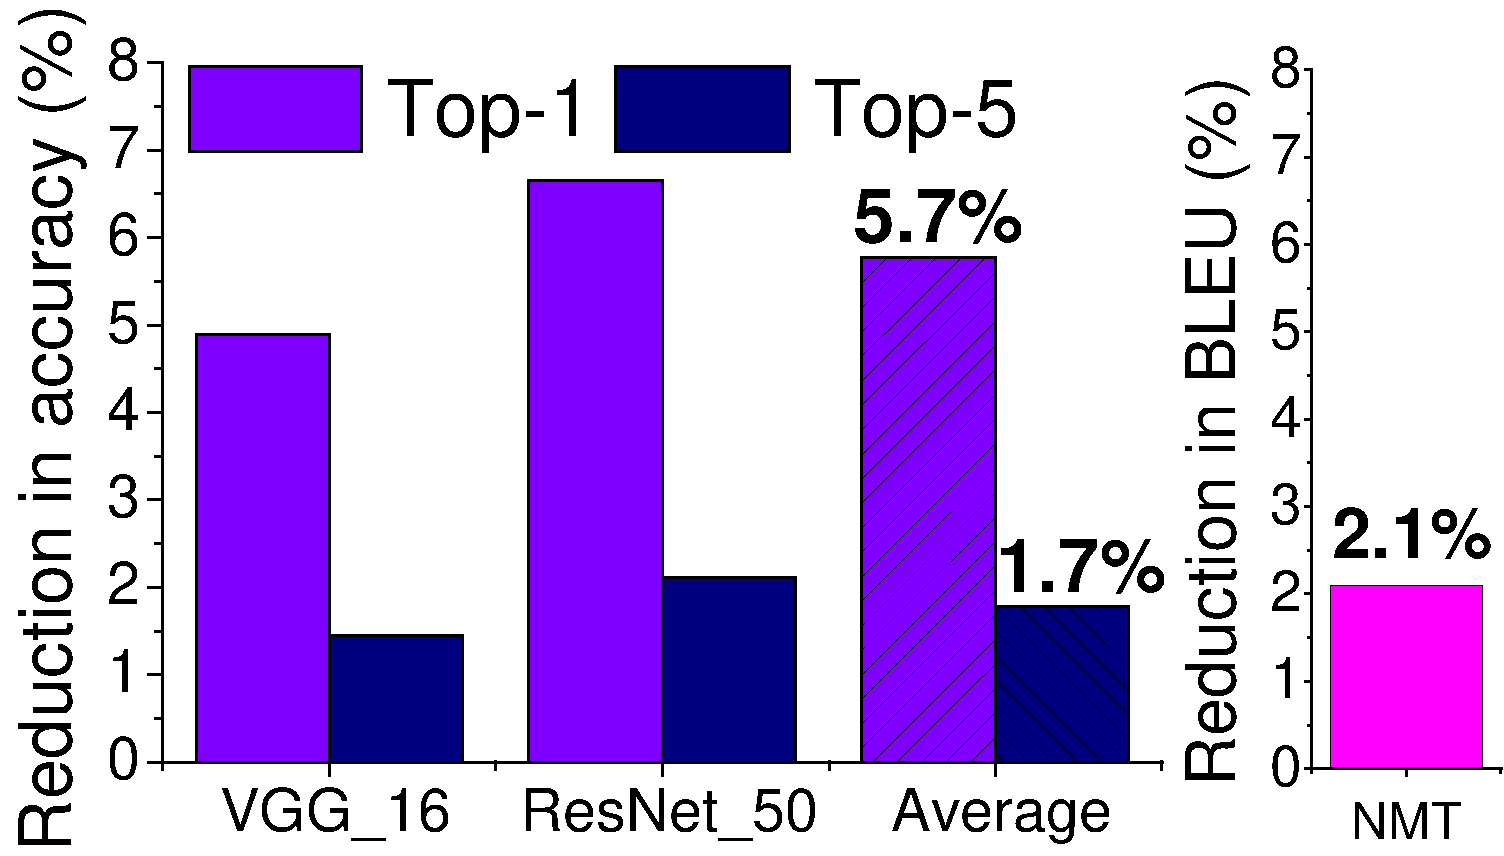
\includegraphics[width=0.3\textwidth]{figure/top1_5_prun.pdf}}
\hfill
\subfloat[][Power consumption]{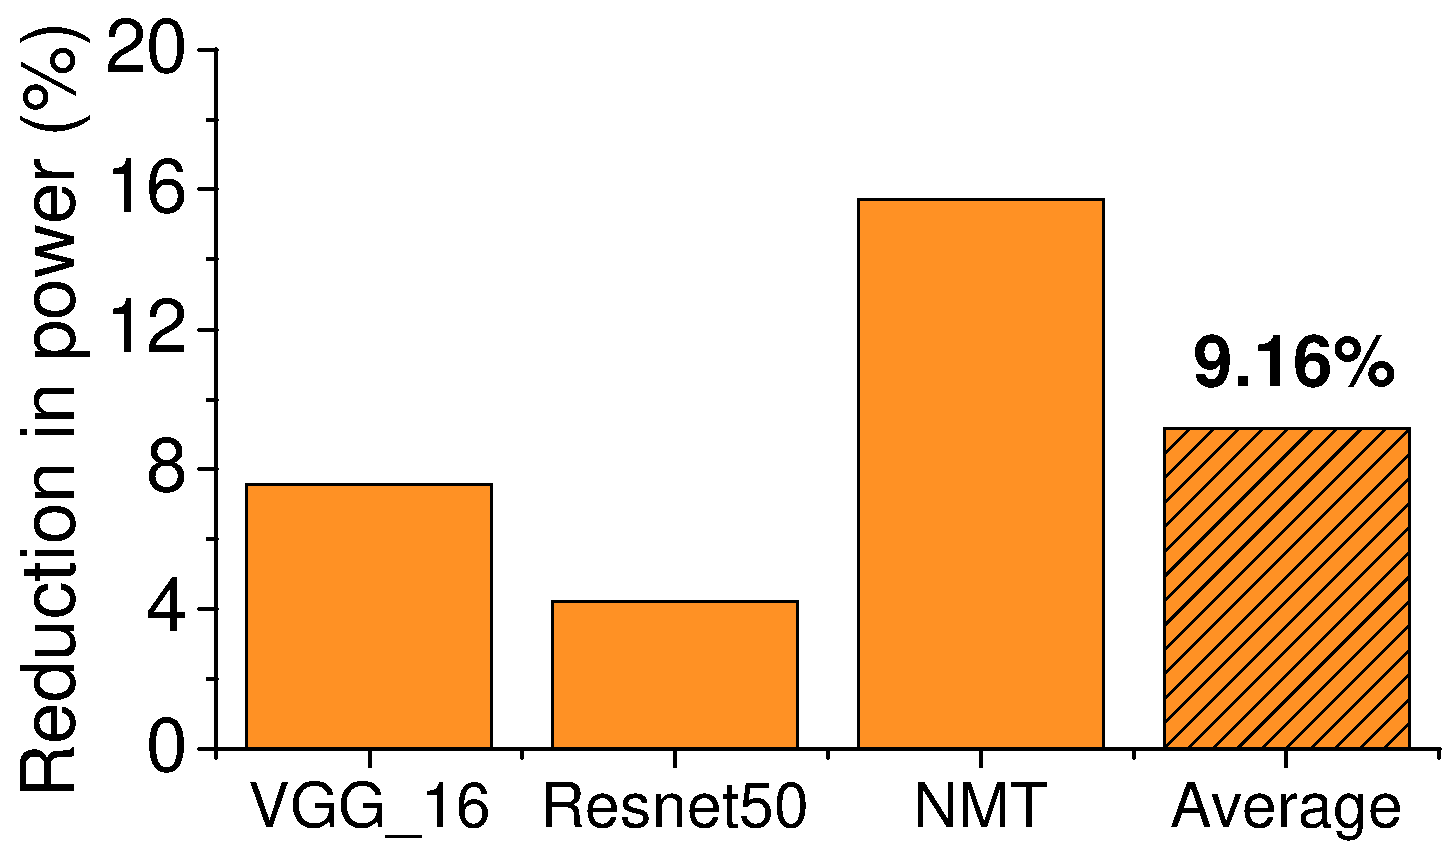
\includegraphics[width=0.3\textwidth]{figure/prun_power.pdf}}
\hfill
\subfloat[][Energy consumption]{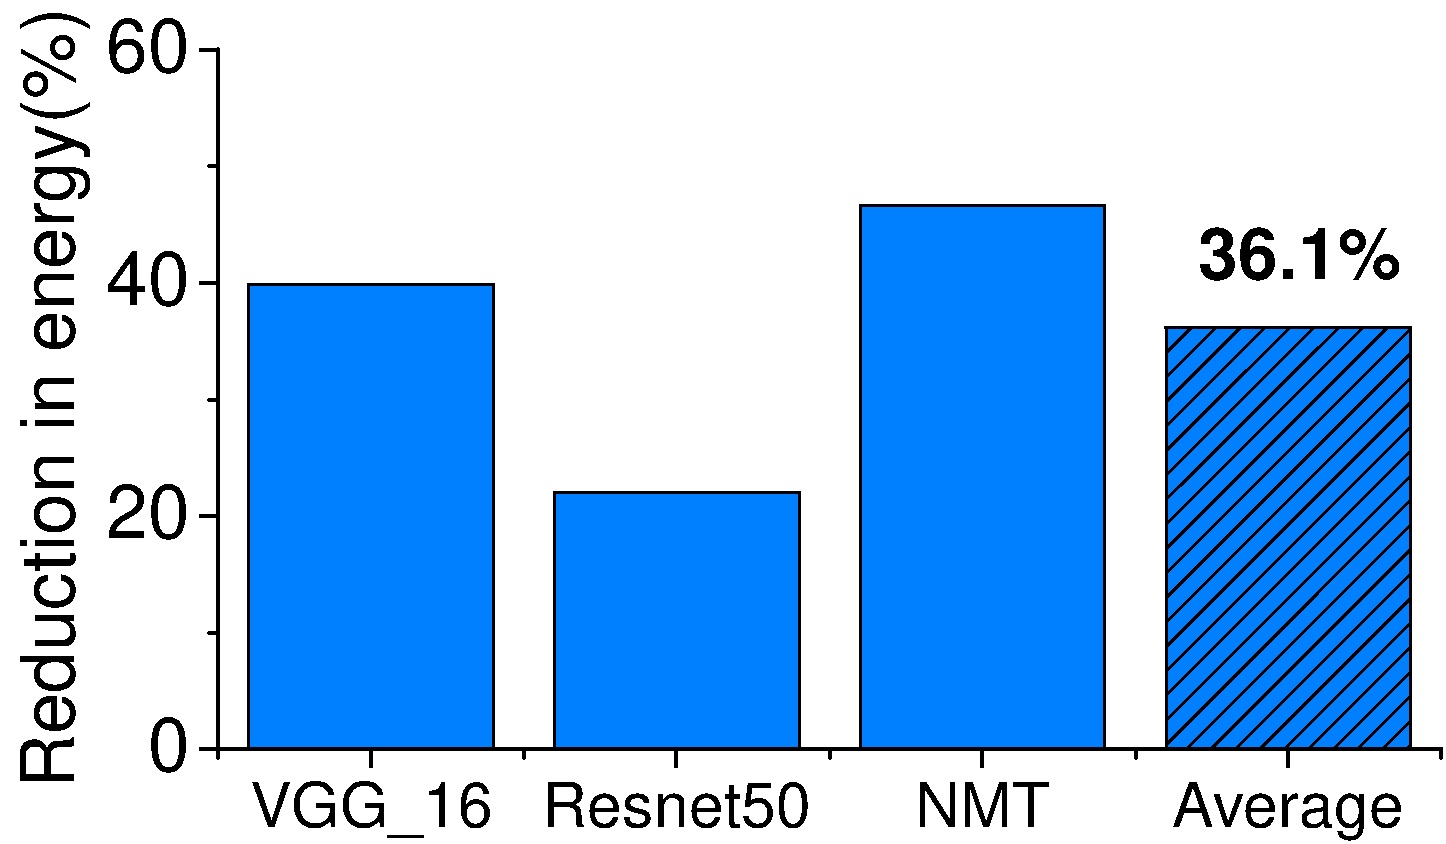
\includegraphics[width=0.3\textwidth]{figure/prun_energy.pdf}}
\hfill

\caption{The achieved model size (a) inference time (b) accuracy/BLEU (c) power consumption (d)
energy consumption (e) and F1 score (e) before and after the compression by \pruning.
The compression technique to use depends on the optimization target.\FIXME{f1 score later}}
\label{fig:analy_prun}
\end{figure*}

\section{Experimental Results}


\subsection{Roadmap}
Our experiments try to answer the following questions:

\begin{itemize}
\item bla
\item bla2
\item bla3
\end{itemize}

\subsection{Impact on the Model Storage Size}
Reducing the model storage size is crucial for embedded and IoT systems which often have a limited storage space. A smaller model size also
translates to smaller runtime memory footprint of less RAM space consumption. Figure~\ref{} illustrates how the different compression
techniques and parameters affect the resulting model size.

Quantization can significantly reduce the model storage size, leading to an average reduction of xx\% (xx MB) and up to xx\% (xx MB). This
compression technique is particularly effective for xx and xx models, because it can xx. From Figure xx (b), we see that the fewer bits
used to represent a weight, the more reduction in the model size we will gain. This is not a surprising as the data width strongly
correlates to the storage size of the model.


Pruning can also reduce the model size, although the gain is smaller than \quantization -- on average xx\% or xx MB (up to xx\% or xx MB).


\subsection{Impact on Accuracy Metrics}
When compressing a model, we still want to largely maintain the performance of a compressed model. Therefore, it is importance to
effectively trade precision for storage space. Results in Figure~\ref{} compare how the prediction accuracy metrics are affected by model
compression.

We see that the sweat spot of \quantization depends on the neural network structure. Although an 8-bit representation leads to a minor
decrease in the prediction accuracy, a further reduction of a 6-bit representation is only profitable for xx networks.

\subsection{Impact on Inference Time}


\subsection{Impact on the Energy Consumption}
